% !TeX spellcheck = es_ES
%----------------------------------------------------------------------------------------
%	PACKAGES AND OTHER DOCUMENT CONFIGURATIONS
%----------------------------------------------------------------------------------------

\documentclass[fleqn,10pt]{SelfArx} % Document font size and equations flushed left
%\usepackage{chemmacros}
\usepackage{ifthen}
\usepackage{calc}
\usepackage{microtype}
\usepackage{ifpdf}
\usepackage[utf8]{inputenc}
\usepackage{amsmath, amsfonts, amssymb}
\usepackage{graphicx, xcolor}
\usepackage{booktabs}
\usepackage{fancyhdr}
\usepackage{lastpage}
\usepackage{titlesec}
\usepackage{titletoc}
\usepackage{enumitem}
%\usepackage{cuted}
\usepackage[version=3]{mhchem}
\usepackage{graphbox}
\usepackage{tabularx}
%----------------------------------------------------------------------------------------
%	COLUMNS
%----------------------------------------------------------------------------------------

\setlength{\columnsep}{0.55cm} % Distance between the two columns of text
\setlength{\fboxrule}{1pt} % Width of the border around the abstract

%----------------------------------------------------------------------------------------
%	COLORS
%----------------------------------------------------------------------------------------

\definecolor{color1}{RGB}{0,94,157} % Color of the article title and sections
\definecolor{color2}{RGB}{255,243,210} % Color of the boxes behind the abstract and headings

%----------------------------------------------------------------------------------------
%	HYPERLINKS
%----------------------------------------------------------------------------------------

\usepackage{hyperref} % Required for hyperlinks
\hypersetup{hidelinks,colorlinks,breaklinks=true,urlcolor=color2,citecolor=color1,linkcolor=color1,bookmarksopen=false,pdftitle={Title},pdfauthor={Author}}

%----------------------------------------------------------------------------------------
%	ARTICLE INFORMATION
%----------------------------------------------------------------------------------------

\JournalInfo{L. de Qu\'imica inorg\'anica II, No. 8, 2016-20} % Journal information
%\Archive{Additional note} % Additional notes (e.g. copyright, DOI, review/research article)

\PaperTitle{Complejos met\'alicos con sacarina} % Article title

\Authors{Juan Barbosa{\color{color1}\textsuperscript{1}\textsuperscript{,2}*},
	Alejandro Camacho{\color{color1}\textsuperscript{1}\textsuperscript{,3}**}} %
%Authors
\affiliation{{\color{color1}\textsuperscript{1}}\textit{Departamento de Qu\'imica, Universidad de los Andes, Bogot\'a, Colombia}} % Author affiliation
\affiliation{{\color{color1}\textsuperscript{2}}\textit{Departamento de F\'isica, Universidad de los Andes, Bogot\'a, Colombia}} % Author affiliation
\affiliation{{\color{color1}\textsuperscript{3}}\textit{Departamento de	F\'isica, Universidad Nacional, Bogot\'a, Colombia}}
\affiliation{{\color{color1}*}\textbf{Email}: js.barbosa10@uniandes.edu.co} %
%Corresponding author
\affiliation{{\color{color1}**}\textbf{Email}: a.camacho10@uniandes.edu.co}
\Keywords{cobre, cobalto, sacarina, compuestos de coordinaci\'on, UV-vis} %
%Keywords - if you don't want any simply remove all the text between the curly
%brackets
\newcommand{\keywordname}{Keywords} % Defines the keywords heading name

%----------------------------------------------------------------------------------------
%	ABSTRACT
%----------------------------------------------------------------------------------------
\Abstract
{
	Los complejos met\'alicos de sacarina: tetraacuo-bis(o-sulfobenzoimido) cobre (II) y tetraacuo-bis(o-sulfobenzoimido) cobalto (II) son sintetizados a partir del sacarinato de sodio, sulfato de cobre pentahidratado y cloruro de cobalto hexahidratado. Los compuestos obtenidos son analizados usando UV-vis en dimetilformamida como solvente, mostrando los m\'aximos de absorbancia en 787 nm y 524 nm correspondientemente. Dichos valores son an\'alogos a los reportados en la literatura. Los rendimientos de la reacci\'on son: 78.24 \% y 74.76 \%, para el cobre y cobalto. La energ\'ia del campo de ligandos se determina en $1.58$ y $2.37$ eV correspondientemente.
}
%----------------------------------------------------------------------------------------

\begin{document}
	\flushbottom % Makes all text pages the same height
	\maketitle % Print the title and abstract box
	%\tableofcontents % Print the contents section
	\thispagestyle{empty} % Removes page numbering from the first page
	%----------------------------------------------------------------------------------------
	%	ARTICLE CONTENTS
	%----------------------------------------------------------------------------------------
	\section*{Introducci\'on}
	Los complejos de coordinaci\'on son esp\'ecies qu\'imicas formadas por un ion met\'alico central unido a un grupo de mol\'eculas o iones. La formación del enlace metal ligando puede ser entendida como la reacci\'on entre un \'acido y una base de Lewis.
	
	Con el objetivo de comprender la coordinaci\'on de la sacarina al ion met\'alico es necesario hacer uso de las teor\'ias de estabilizaci\'on de los compuestos de coordinaci\'on, una de ellas es el concepto de dureza de Pearson. Seg\'un esta teor\'ia los compuestos de coordinaci\'on son m\'as estables cuando los enlaces se realizan entre \'acidos y bases de la misma dureza. Se denominar\'an \'acidos duros a aquellos compuestos con peque\~no radio at\'omico, y gran cantidad de carga. En el caso de las bases duras se espera que el compuesto sea poco polarizable \cite{Pearson}.
	
	El o-sulfobenzoimido o sacarina es un compuesto org\'anico arom\'atico con dos grupos polares importantes, el grupo amido y sulfona. Estas caracter\'isticas le otorgan a la sacarina propiedades edulcolantes que permiten su uso como aditivo alimenticio \cite{Saccharine}. El sacarinato corresponde con la base conjugada de la sacarina, el cual se produce al perder un prot\'on como se muestra en el \autoref{sch: saccharine-pka}.
	\begin{scheme}[h]
		\centering
		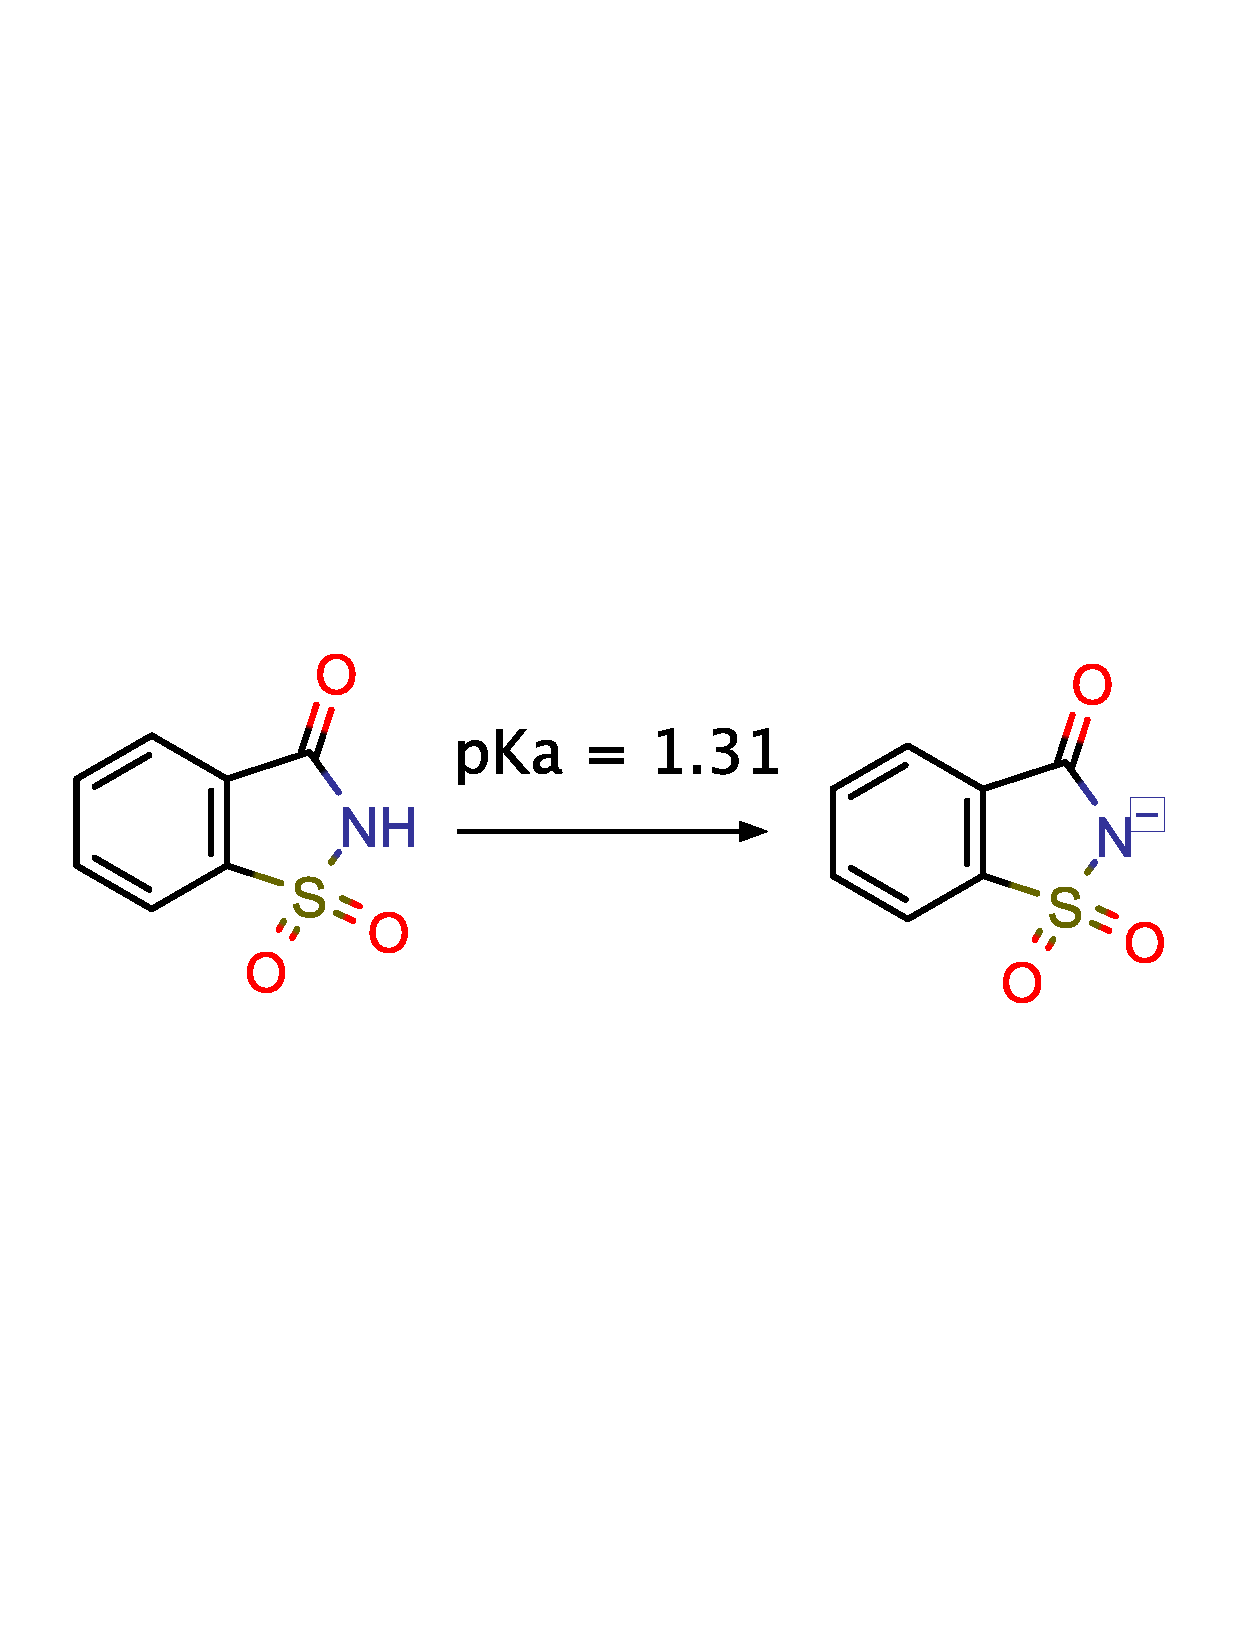
\includegraphics[width=0.7\linewidth]{images/saccharine.pdf}
		\caption{Relaci\'on de la sacarina con su base conjugada, con la constante de acidez reportada \cite{Saccharine}.}
		\label{sch: saccharine-pka}
	\end{scheme}
    
	\section{Metodolog\'ia}
	La metodolog\'ia usada para la s\'intesis de los complejos met\'alicos de sacarina es an\'aloga para ambos metales. En primer lugar se disolvieron 0.5182 g de sulfato de cobre pentahidratado (0.4785 g de cloruro de cobalto hexahidratado) en 60 mL de agua destilada. Posteriormente se agregaron cerca de 1 g de sacarina a cada una. Las soluciones fueron concentradas mediante la evaporaci\'on del solvente con calor y r\'afajas de aire, hasta alcanzar volumenes de 20 y 25 mL correspondientemente. Finalmente las soluciones son enfriadas hasta la cristalizaci\'on en ba\~no de hielo. Los cristales son recuperados por filtraci\'on al vac\'io usando embudos B\"uchner. 
	
	\begin{figure*}[h]
		\centering
		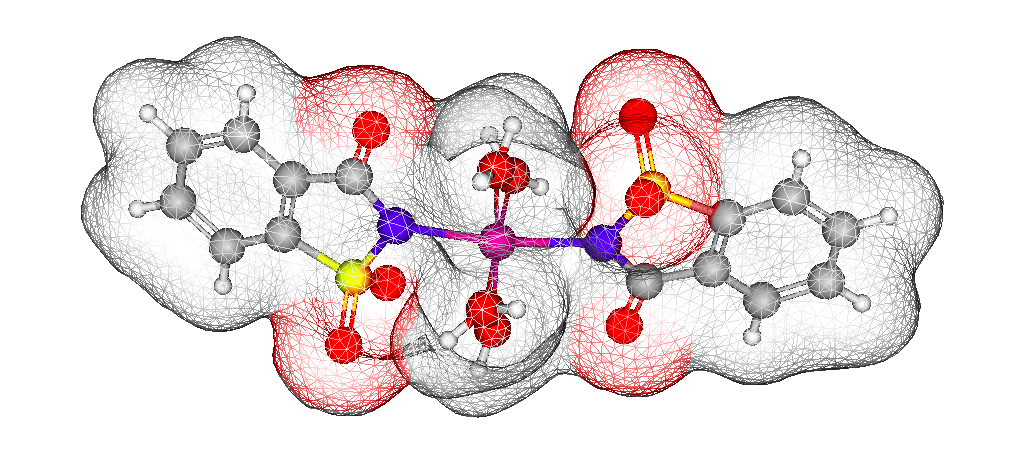
\includegraphics[width=\linewidth]{images/SacarineComplex.png}
		\caption{Estructura qu\'imica del tetraacuo-bis(o-sulfobenzoimido) cobre (II), en rojo se muestran las zonas polares de la mol\'ecula.}
		\label{fig: 3d complex}
	\end{figure*}
	
	\section{Resultados y Discusi\'on}
	Al final de la reacci\'on se obtuvieron masas de producto de 0.8701 g y 0.7987 g para el compuesto con cobre y cobalto correspondientemente. Lo anterior equivale a rendimientos de 78.24 \% y 74.76 \% para las reacciones. Con el objetivo de entender la diferencia en los rendimientos se hace uso de los conceptos desarrollados en la introducci\'on sobre la qu\'imica de coordinaci\'on.
	
	El compuesto se forma a partir de los iones se de cationes met\'alicos y el sacarinato libre. Con el objetivo de aumentar la probabilidad de choques y con ellos la coordinaci\'on se aumenta la temperatura al mismo tiempo que se disminuye el volumen de soluci\'on. Sin embargo no todas las esp\'ecies interactuan de la misma forma con las dem\'as. El r\'adio at\'omico del cobre es de 128 pm mientras el del cobalto es 125 pm, dado que ambos cationes presentan la misma carga, el cobalto (II) se clasifica como un \'acido mas duro que el cobre (II).
	\begin{scheme}[h]
		\centering
		\begin{tabular}{c}
			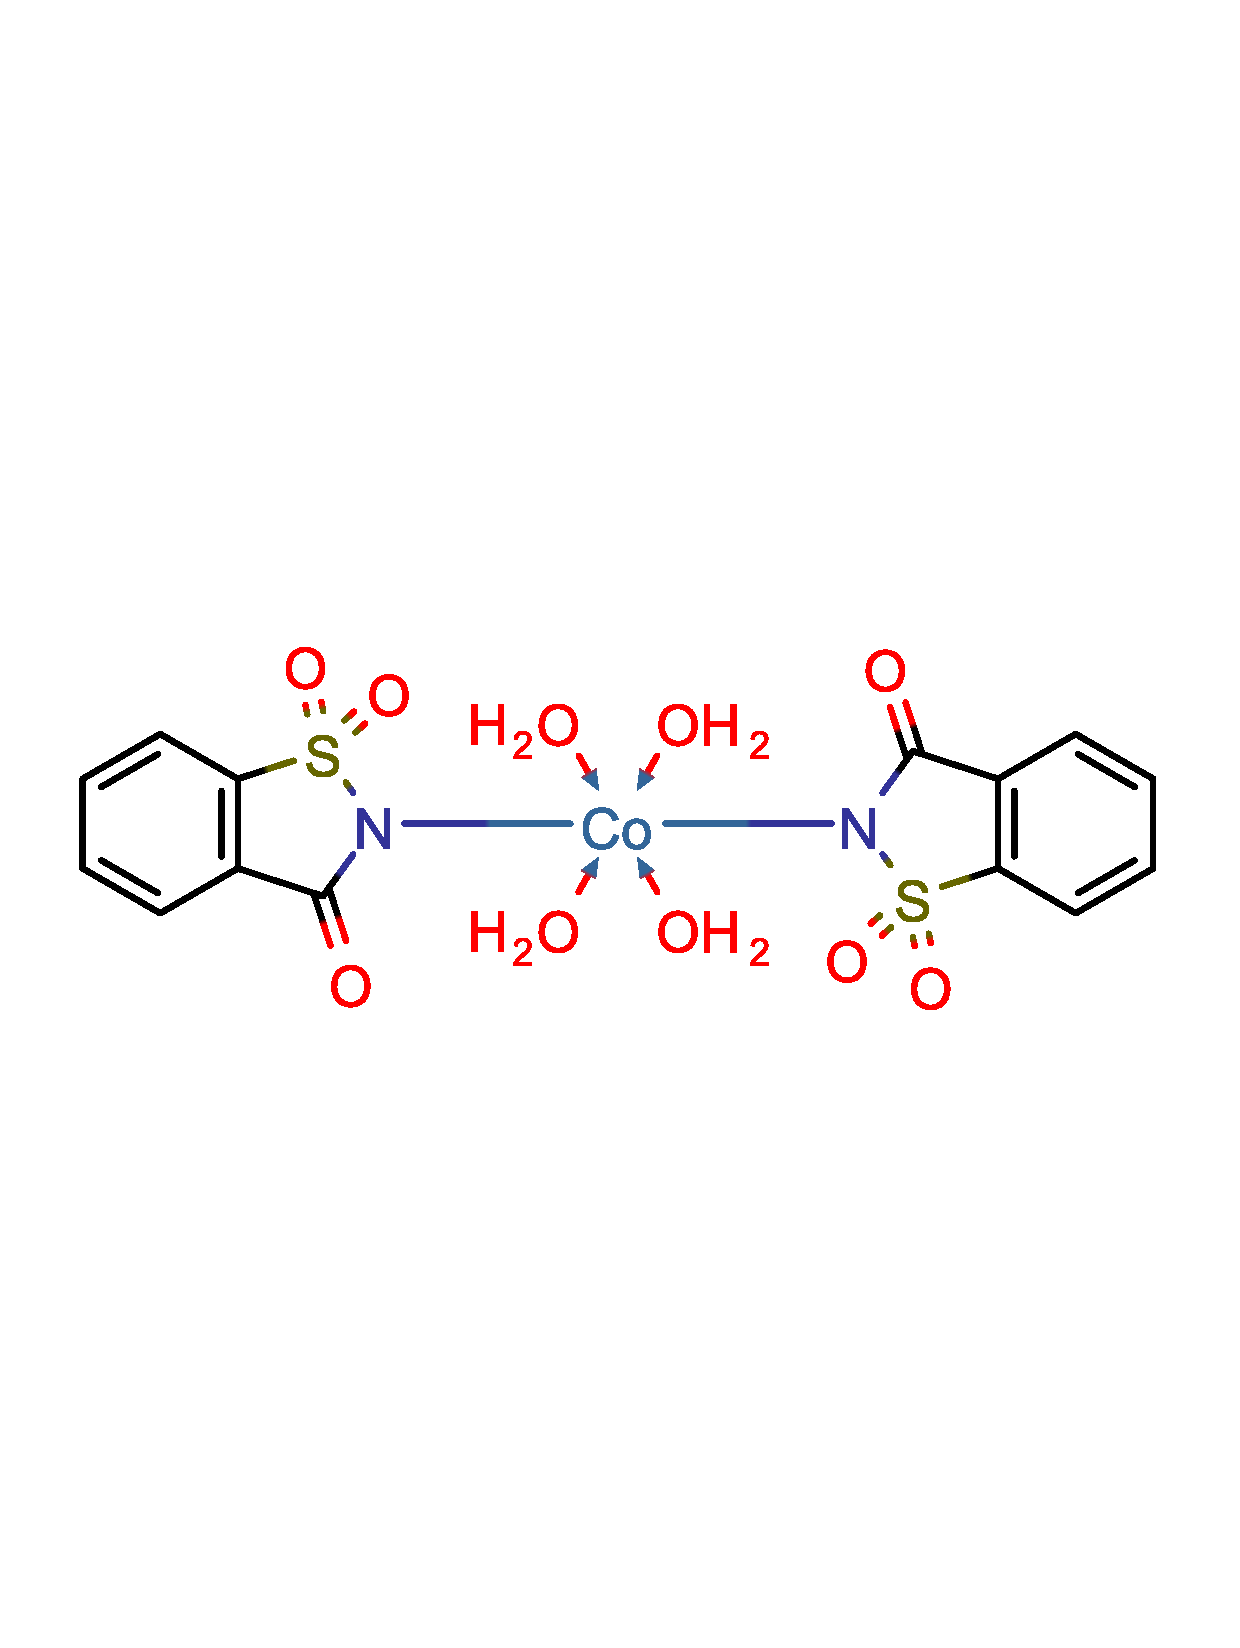
\includegraphics[width=0.7\linewidth]{images/cobalt.pdf} \\
			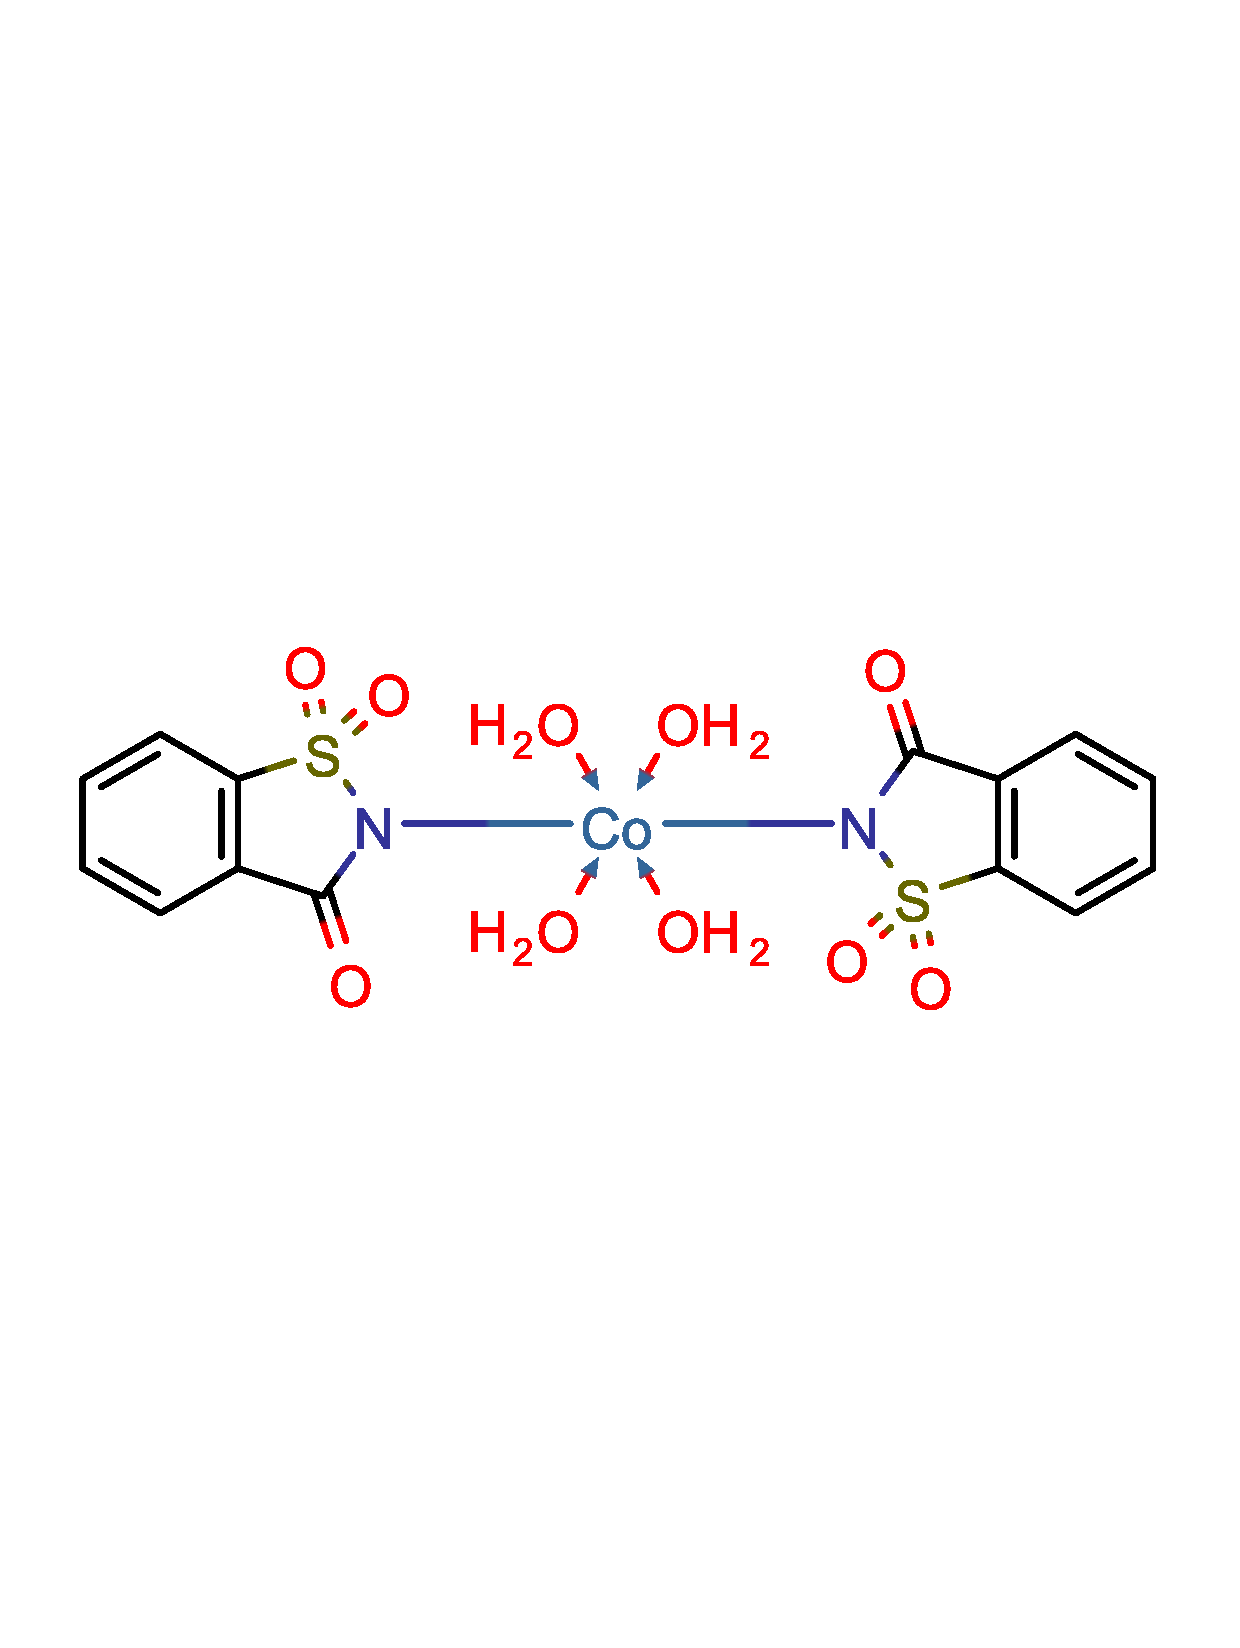
\includegraphics[width=0.7\linewidth]{images/cobalt.pdf}
		\end{tabular}
		\caption{Estructura qu\'imica del tetraacuo-bis (o-sulfobenzoimido) cobre (II) y cobalto (II)}
		\label{sch: complexes}
	\end{scheme}
	
	Si bien ambos metales dan lugar a compuestos parecidos como se muestra en el \autoref{sch: complexes}, uno de los dos es m\'as estable y por ende su s\'intesis se ve favorecida en t\'erminos de rendimiento. Los ligandos para ambos compuestos son los mismos: mol\'eculas de agua en la esf\'era de coordinaci\'on y dos aniones de sacarinato.
	
	Existen al menos dos formas para aproximarse a la dureza del sacarinato. Por un lado se encuentra el concepto de Pearson, en donde la mol\'ecula debe ser poco polarizable para ser considerada una base dura, lo cual no sucede con el sacarinato, dado que toda la carga estar\'a concentrada en el anillo menor. Una segunda forma es considerar la constante de acidez de la sacarina cuyo valor es de 1.31, lo cual implica que se puede considerar un \'acido fuerte, por lo cual su base conjugada ser\'a d\'ebil.
	
	\pagebreak
	Usando el concepto de Pearson se puede establecer entonces el \'orden de estabilidad para los dos compuestos. La estabilidad del compuesto con cobre ser\'a mayor que la del cobalto, dado que los compuestos prefieren coordinarse por pares de dureza. Lo cual da explicaci\'on a las diferencias de rendimiento.
	\begin{figure}[h]
		\centering
		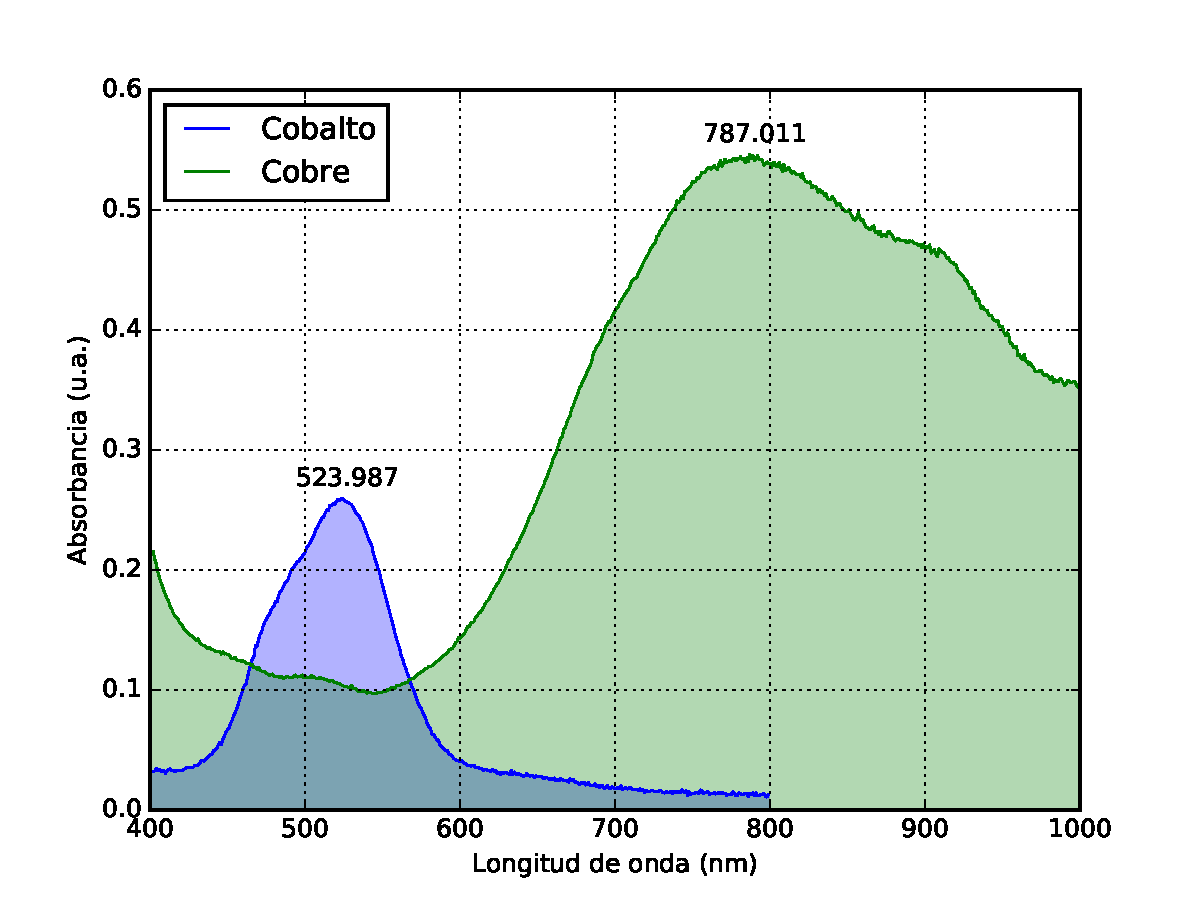
\includegraphics[width=\linewidth]{images/absorbances.pdf}
		\caption{Resultados del an\'alisis por espectroscop\'ia UV-vis.}
		\label{fig: UV-vis}
	\end{figure}
	
	El espectro UV-vis tambi\'en constituye una fuente importante de informaci\'on, puesto que permite identificar los compuestos y determinar la energ\'ia del campo de ligandos. Los espectros de ambos compuestos se pueden observar en la \autoref{fig: UV-vis}. Para ambos se observa una \'unica banda bien resuelta, donde $\lambda_{\ce{Co}} < \lambda_{\ce{Cu}}$. Las bandas cohinciden con lo reportado en la literatura para los complejos sintetizados.

	Es posible determinar la energ\'ia del campo de ligandos $\Delta_0$ usando la energ\'ia de una onda electromagn\'etica:
	\begin{equation}
		E = \Delta_0 = h\nu = h\dfrac{c}{\lambda}
	\end{equation}
	
	Los valores de energ\'ia del campo de ligandos son entonces $\Delta_{0\ce{Cu}} = 1.58$ eV y $\Delta_{0\ce{Co}} = 2.37$ eV. Si se tiene encuenta adem\'as que los sistemas f\'isicos buscan el estado de m\'inima energ\'ia, la informaci\'on sobre el campo de ligandos permite explicar tambi\'en la estabilidad relativa entre los dos compuestos.
	
	Finalmente una cosa que se debe tener en cuenta respecto a las posiciones de coordinaci\'on es que los dos ligandos de sacarinato deben quedar lo m\'as distantes posibles para evitar interacciones electroest\'aticas desfavorables por los grupos electronegativos en el compuesto como se observa en la \autoref{fig: 3d complex}. Donde los ligandos acuo ocupan las posiciones ecuatoriales y los ligandos voluminosos las axiales.
	
	\section{Conclusiones}
	Los rendimientos de las s\'intesis de los complejos de sacarina se determinaron en 78.24 \% y 74.76 \% para el cobre y cobalto correspondientemente. Adicionalmente se determin\'o la energ\'ia del campo de ligandos en 1.58 y 2.37 ev. Usando conceptos te\'oricos tales como el concepto de \'acidos blandos y duros de Pearson, la polarizaci\'on en mol\'eculas org\'anicas y la teor\'ia de compuestos de coordinaci\'on fue posible comprender los rendimientos obtenidos en la s\'intesis as\'i como los resultados espectrosc\'opicos en el rango UV-vis.
	\phantomsection
	\bibliographystyle{unsrt}
	\begin{thebibliography}{9}
		\bibitem{Pearson}
		Singh, D. N.; Harbaugh, W. H. \textit{Basic concepts of inorganic chemistry}; Pearson: United States, 2011.
	    \bibitem{Saccharine}
	    Medina, D. A. V.; Ferreira, A. P. G.; Cavalheiro, E. T. G. Thermal investigation on polymorphism in sodium saccharine. \textit{Journal of Thermal Analysis and Calorimetry}. Published Online: March 22, 2014, 117 (\textit{1}), 361–367.
	\end{thebibliography}
\end{document}
